\chapter {Quick Reference: Component Details}
\section{BJT BF194/195}
\label{BF194/195}
BF194/195 is a high frequency transistor. From its datasheet 

Type Designator: BF194/BF195

Material of transistor: Si

Polarity: NPN

Maximum collector power dissipation ($Pc$), W: 0.25

Maximum collector-base voltage |$V_{cb}$|, V: 30

Maximum collector-emitter voltage |$V_{ce}$|, V: 20

Maximum emitter-base voltage |$V_{eb}$|, V: 5

Maximum collector current |$I_{c max}$|, mA: 30

Forward current transfer ratio (hFE), min: 67

\textcolor{red}{TODO: Pinout diagram to be added}
\section{BJT BC107}
\label{BC107}
Type Designator: BC107

Material of transistor: Si

Polarity: NPN

Maximum collector power dissipation ($P_c$), W: 0.3

Maximum collector-base voltage |$V_{cb}$|, V: 50

Maximum collector-emitter voltage |$V_{ce}$|, V: 45

Maximum emitter-base voltage |$V_{eb}$|, V: 6

Maximum collector current |$I_{cmax}$|, A: 0.1

Forward current transfer ratio ($h_{FE}$), min: 110

Package of BC107 transistor: TO18
\textcolor{red}{TODO: add schematic diagram and photo of BC107}

\section{Intermediate Frequency Transformer}
\label{IFT}
IF Taransformers come as specially designed tuned circuits in groundable metal packages called IF cans. The primary winding has an inducance of $L_{eq}=450\mu H$ and it comes with a shunt capacitor of capacitance $C=270\ pF$. Its resonant frequency is thus $f=\frac{2\pi}{\sqrt{L_{eq}C}}\approx 455 kHz$.\\ This frequecy is adjustable by a factor of $\pm 10 \%$ . IFT has a tapped primary winding as shown in the schematic diagram, figure \ref{iftschem}. 

The ferrite core between primary and secondary windings is tunable with a non-metallic screw driver or tuning tool. It changes the mutual inductance and thus control the Q-factor of the collector circuit of connected transistor\cite{Tomasi}.
 
\begin{figure}
\centering{ 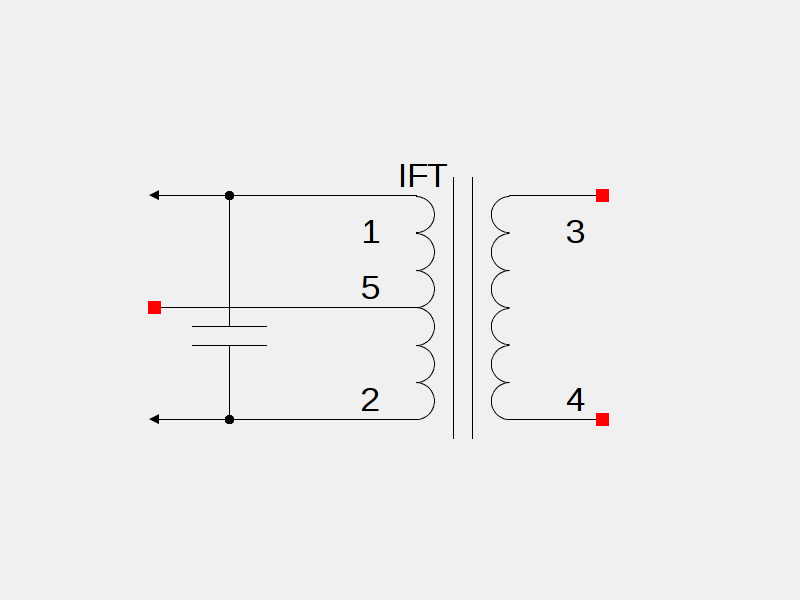
\includegraphics[width=7cm, height=5cm, trim= 2cm 2cm 2cm 2cm, clip=true]{IFT.png}}
\caption {Schematic Diagram of Intermediate frequency Transformer}
\label{iftschem}
\end{figure}

\textcolor{red}{TODO: add photo of IFT}


\section{AD 633 - Multiplier IC}
\label{AD633}
\paragraph{Multiplier ICs:}
 Analog multipliers are complex arrangements of Opamps and other circuit elements in the form of IC. It can be used for different applications like multiplication, division, squarer, modulator, demodulator, filter etc. There are two inputs $\textbf{X}$ and $\textbf{Y}$ to which the signals to be multiplied are given.
There are two input terminals $\textbf{X}$ and $\textbf{Y}$ to which the signals to be multiplied are given. The output W is the product of instantaneous values of input signals reduced by a scale factor $\textbf{k}$. $\textbf{k}$ is usually less than 1. For practical ICs $\textbf{k}=\frac{1}{10}$.

\begin{equation}
W=kXY
\end{equation}

\begin{figure}[h]
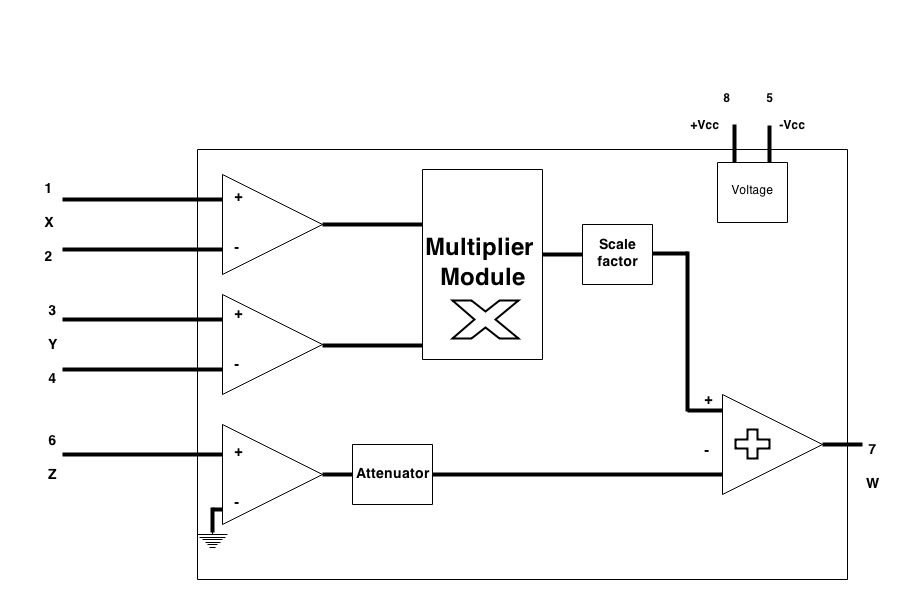
\includegraphics[width=10cm, height=7cm]{ad633.png}
\caption{Functional Block Diagram for AD633 multiplier IC}
\label{ad633}
\end{figure}

\paragraph{AD633} is functionally a complete four quadrant analog multilier IC. The functional block diagram is shown in Fig. \ref{ad633}. This IC uses Gilbert's transconducatnce multiplier module in four quadrants. On chip circuit provides a scale factor of $k=\frac{1}{10}$. If $\textbf{X}$, $\textbf{Y}$ and $\textbf{Z}$ inputs are given we get 
\begin{equation}
W=\frac{XY}{10}+Z
\end{equation}

Here $\textbf{Z}$ is the input to the summing amplifier. If the summing amplifier input is grounded, then output 
\begin{equation}
W=\frac{XY}{10}
\end{equation}

\paragraph{Specifications}as in AD633 data sheet is,

\noindent Dual power supply: $V_{cc}= \pm \ 8V to \pm \ 18V$

\noindent Input impedance > $5 M \Omega$

\noindent Output impedance < $75  \Omega$

\noindent Maximum operating frequency (Bandwidth) = $1 M\Omega$

